%----------------------------------------------------------------------------
\chapter{\kli}
%----------------------------------------------------------------------------
\section{Tervezés}
A tervezés legelső fázisában meg lett határozva, hogy milyen problémát szeretnék megoldani.
Ennek a projektnek az volt a célja, hogy létrehozzon egy felhasználóbarátabb lehetőséget istio operátor telepítésére és ezen feladatokon keresztül megismerkedjem a kubernetes müködésével go programozási nyelven keresztül.
Fontos szempont volt, hogy a program felépítése moduláris legyen és könnyen hozzáférhető, ami a továbbfejlesztését teszi lehetővé ennek a programnak.

A tervezés következő fázisa a megvalósításhoz szükséges eszközök, erőforrások és elméleti anyagok összegyűjtése volt.
Ezeknek az anyagoknak az összegyűjtése kihívásokkal járt, mert az interneten fellelhető cikkek közül rengeteg volt elavult.

A programozási nyelv választása egyszerű feladatnak bizonyult, ugyanis elterjedt a go programozási nyelv használata mikroszolgáltatások körében.
Széleskörű könyvtár választék állt rendelkezésre a kubernetes API szerver kommunikáció lebonyolítására, helm chart telepítésére, yaml fájlok beolvasására és kezelésére.
Szintaktikája hasonló a C és Python programozási nyelvekhez, így hamar sikerült elsajátítanom.

A tervezés utolsó fázisában került elő a program felépítésének kialakítása.
Kettő logikai részre osztottam a CLI-t, ami kli és kubereflex csomagokként jelenik meg.
Ennek célja a felület és logika kódjának szeparálása, így egyszerűbb fejlesztést és tesztelést tesz lehetővé.

\section{Model-View-Controller ismertetése}
A Model-View-Controller (későbbiekben MVC) programtervezési mintát használtam a fejlesztéskor ahogy az a \ref{kli-mvc} ábra is szemlélteti.
Ez a model segített abban, hogy szétválasszam a nézet réteget az adatrétegtől.
A két réteg közötti kommunikációt egy vezérlői réteg oldja meg.
Itt történik az adatok átadása, validálása az üzleti logika segítségével.
Mivel a modulok a projetkben függetlenek egymástól köszönhetően az MVC alkalmazásának, így könnyű volt a későbbiekben változtatni és bővíteni az egyes modulok viselkedését.
A tesztelhetőséget is nagyban megkönnyítette, mivel lehetőség adódott szimulálni (mock-olni) egy adott modult a másik modul tesztelésekor.

\begin{figure}[ht]
  \centering
       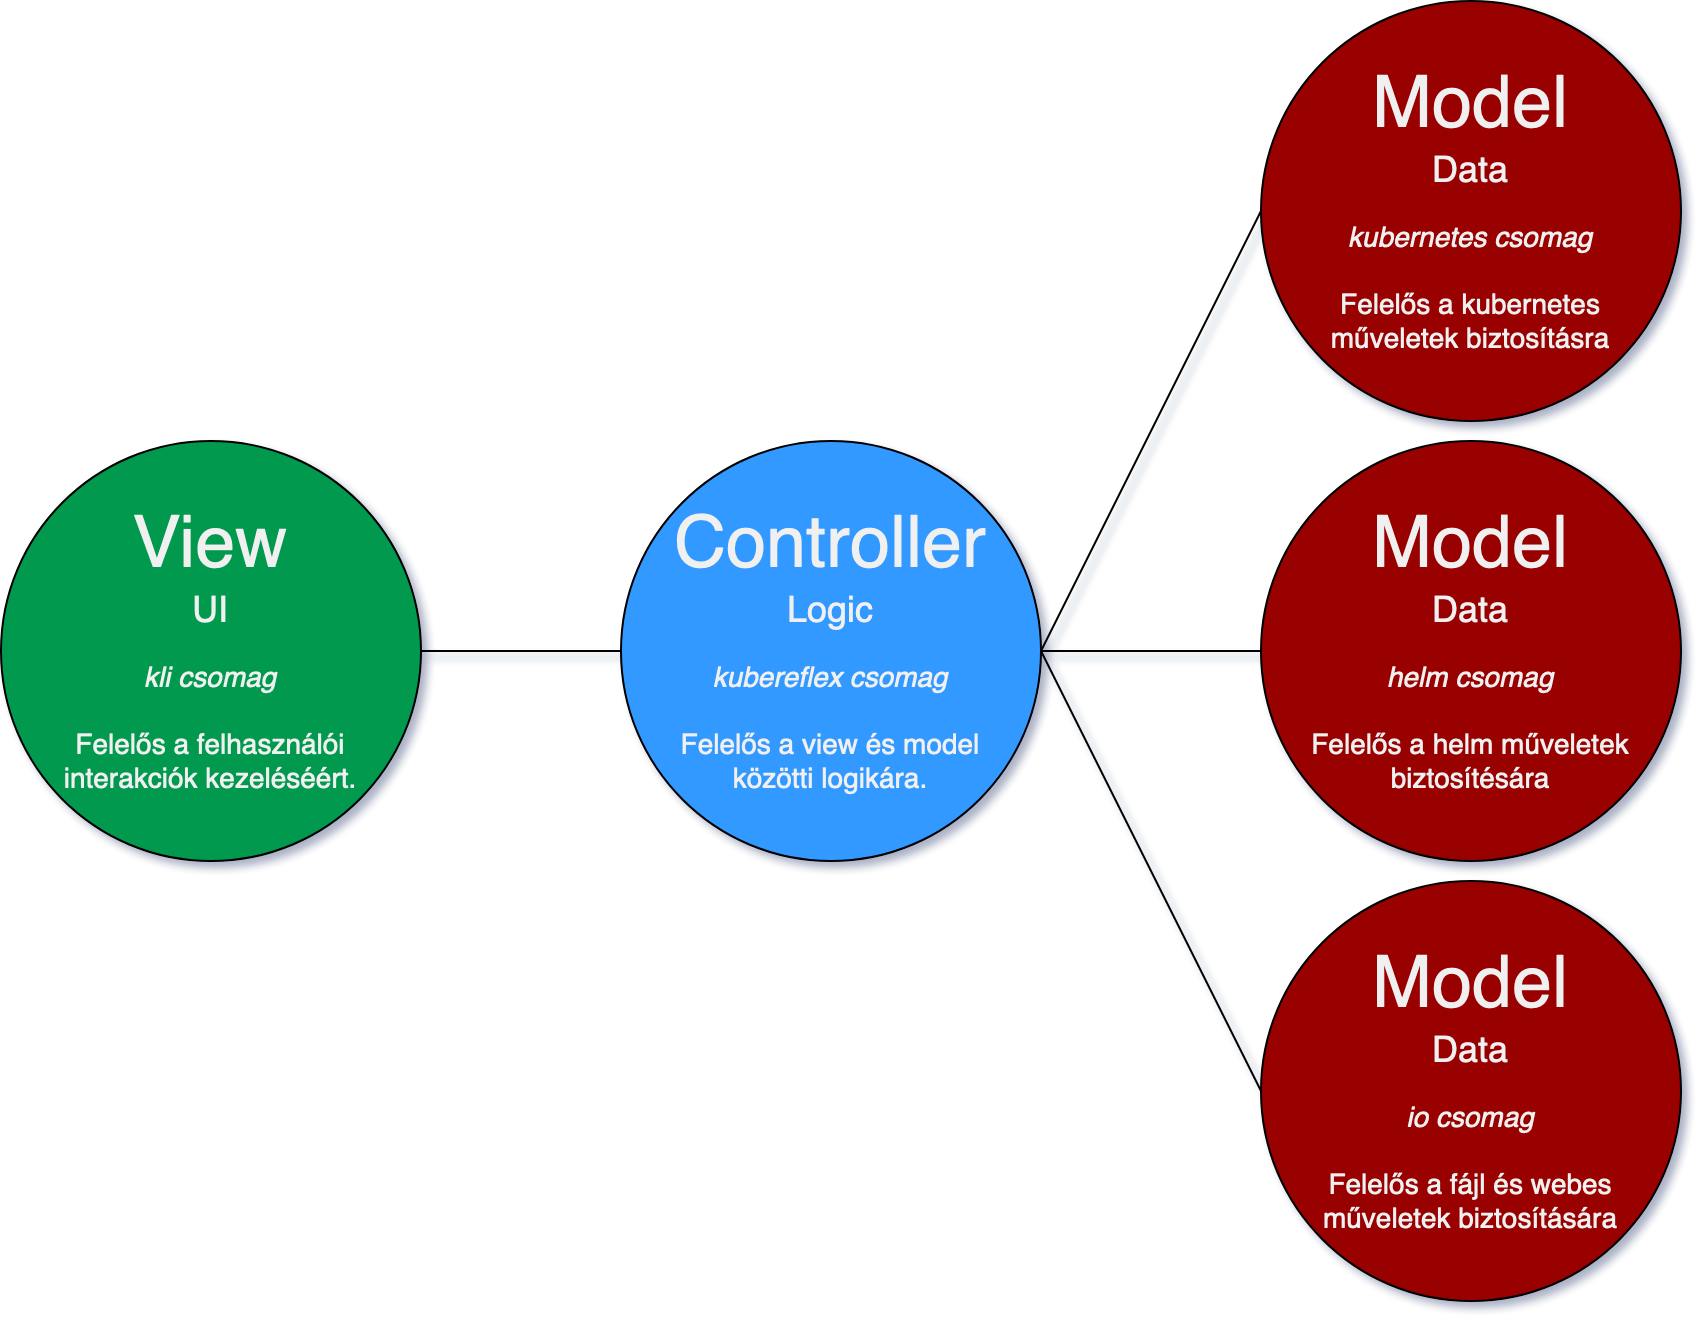
\includegraphics[width=1.0\textwidth]{figures/kli/kli-mvc.png}
        \caption{Diagram a projekt felépítéséről}
         \label{kli-mvc}
\end{figure}

\section{Megvalósítás}

\subsection{CLI keretrendszer}
A CLI funkciók implementálását nagyban felgyorsította spf13 felhasználó által fejlesztett cobra könyvtár.
Ez a könyvtár csomag egy keretrendszert biztosít a konzolos applikációk fejlesztéséhez és biztosít könnyen generálható cobra alkalmazásokat.
Ez a generált alkalmazás funkció egy könnyen érthető és bővíthető vázat kínált számomra, amit kibővítettem a saját kódommal.

Használata egyszerű volt, mivel a go csomagkezelővel könnyedén telepíthető a cobra.
A telepítés után a cobra init parancs legenerálta a váz kódot és a cobra add parancs adta hozzá a parancsokat ehhez a vázhoz.
Ezt a kiindulási kód csomagot neveztem el kli-nek.

\newpage

A kli csomag felel a felhasználói felület kezeléséért mint például:
\begin{itemize}
    \item Flag-ek kezelése.
    \item Interaktív kontextus választó menü.
    \item Felhasználói visszajelzések a folyamatokról üzenetek formájában.
    \item Segítség a konzolos parancsok használatához.
\end{itemize}

Az install és uninstall parancsokhoz tartoznak flag-ek, melyekkel konfigurálni lehet bizonyos paramétereit az adott parancsnak.
Az install és uninstall flag-ek rövid ismertetése:
\begin{itemize}
    \item \texttt{-{}-}main-cluster vagy \texttt{-}c segít az elsődleges cluster konfigurációs fájl elérési útvonalának megadásában.
    \item \texttt{-{}-}secondary-cluster vagy \texttt{-}C segít az másodlagos cluster konfigurációs fájl elérési útvonalának megadásában.
    \item \texttt{-{}-}main-context vagy \texttt{-}k segít az elsődleges cluster kontextus nevének megadásában.
    \item \texttt{-{}-}secondary-context vagy \texttt{-}K segít az másodlagos cluster kontextus nevének megadásában.
    \item \texttt{-{}-}active-custom-resource vagy \texttt{-}r segít az elsődleges cluster istio control plane resource konfigurációs fájl elérési útvonalának megadásában.
    \item \texttt{-{}-}passive-custom-resource vagy \texttt{-}R segít az másodlagos cluster istio control plane resource konfigurációs fájl elérési útvonalának megadásában.
    \item \texttt{-{}-}attach vagy \texttt{-}a segít a kettő megadott cluster-t összekapcsolni.
    \item \texttt{-{}-}detach vagy \texttt{-}d segít a kettő megadott cluster-t szétválasztani.
    \item \texttt{-{}-}verify vagy \texttt{-}v segít a telepített resource-ok helyességének ellenőrzésében.
    \item \texttt{-{}-}timeout vagy \texttt{-}t segít beállítani a várakozási időt egy resource telepítésénél.
    \item \texttt{-{}-}help vagy \texttt{-}h segít leírni a parancsokat.
\end{itemize}

Használati példák:
\begin{itemize}
    \item kli install \texttt{-{}-}active-custom-resource istio\texttt{\_}a\texttt{\_}resource.yaml \texttt{-{}-}passive-custom-resource istio\texttt{\_}p\texttt{\_}resource.yaml \texttt{-{}-}attach \texttt{-{}-}verify \texttt{-{}-}timeout 90
    \item kli uninstall \texttt{-{}-}active-custom-resource istio\texttt{\_}a\texttt{\_}resource.yaml \texttt{-{}-}passive-custom-resource istio\texttt{\_}p\texttt{\_}resource.yaml \texttt{-{}-}detach
\end{itemize}

Amikor meghívjuk az install flag-ek akkor a telepítés előtt ellenőrzés zajlik le, majd egy repository hozzáadás és frissítés.
Ezután települ fel a helm csomag.
A célja ennek a front-end csomagnak, hogy minimalizálja a függőségeit a külső moduloktól és csak a kubereflex back-end csomag funkcióira támaszkodjon.

\subsection{Controller bemutatása}
A kubereflex csomag felépítése modulárisra lett tervezve.
A csomag fő modulja arra szolgál, hogy publikusan elérhetővé tegye az amúgy privát funkciókat az almodulokból és egy kontroller szerepet töltsön be.
Itt található a üzleti logika, az adatok átadása és a hibák kezelése is.

A következő szekciókban az kubereflex almoduljait fogom bemutatni.

\subsubsection*{helm almodul}
Ez az almodul felel az összes olyan funkcióért, amit a Helm csomagkezelővel szeretnénk végrehajtani.
Példaképpen felhozható az előre kész helm chart applikáció telepítése, törlése, repository hozzáadása és frissítése.
Egy chart telepítésének folyamata látható a \ref{helm-simple-sequence} ábrán.
Ahhoz, hogy egy chart telepíthető legyen elő kell készíteni egy helm klienst.
Ezután a helm kliens használatával frissíteni kell a lokális repository konfigurációnkat, ahonnan majd elérhető lesz a telepíteni kívánt chart.
Létre kell hozni egy telepítési cselekvést (későbbiekben action), ami leírja részletesen a chart adatait. Ilyen adatnak tekinthető a kiadási név (későbbiekben release name), opcionális paraméterek a chart-nak, helm kliens verziószáma és melyik névtérbe (későbbiekben namespace) legyen telepítve a chart.
Ez az action kérés fog átadásra kerülni a helm kliensnek, amely azt feldolgozza.

\begin{figure}[ht]
    \centering
         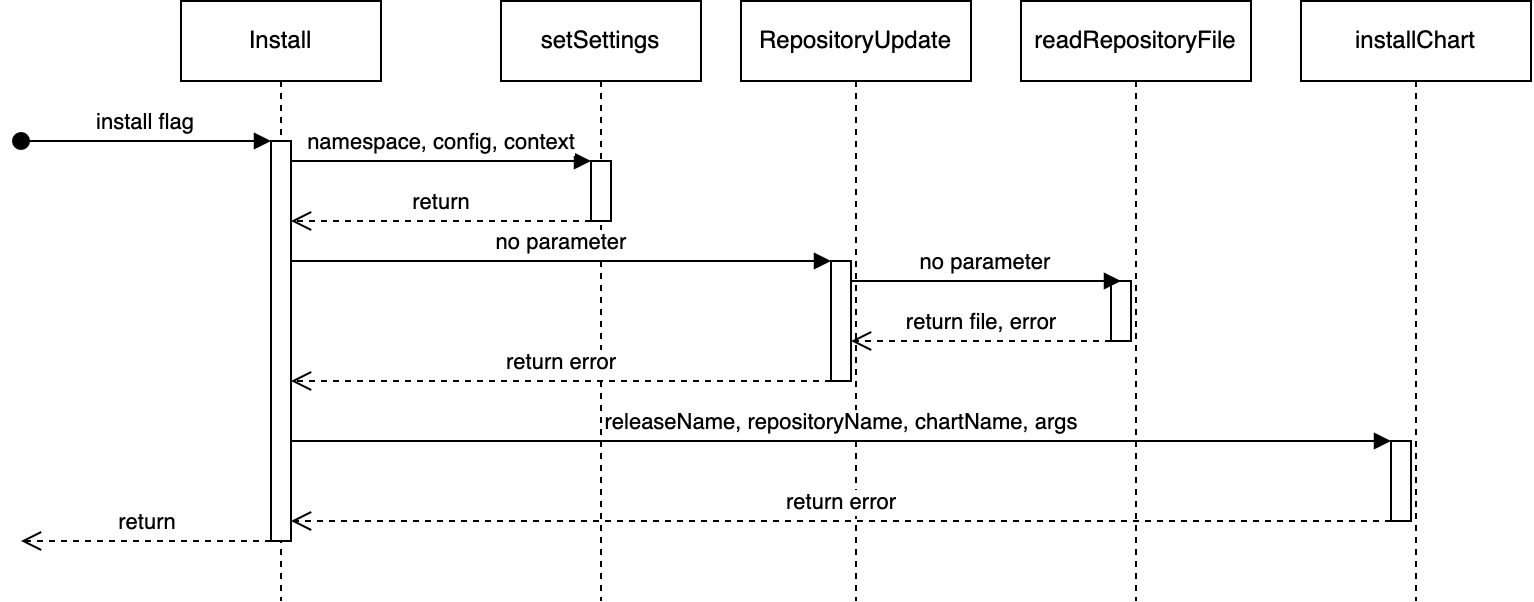
\includegraphics[width=1.0\textwidth]{figures/kli/helm-simple-sequence.png}
          \caption{Egyszerűsített diagram a helm chart telepítési folyamatáról.}
           \label{helm-simple-sequence}
\end{figure}

A következő metódusok funkcióinak összefoglalása:
\begin{itemize}
    \item setSettings metódus felel a helm kliens névterének, kubernetes konfigurációs fájl beállításáért és a kubernetes kontextus megadásáért.
    \item Install metódus feladata, hogy meghívja a szükséges függvényeket a telepítés lefuttatása előtt és hiba esetén térjen vissza a hiba okával.
    \item RepositoryUpdate metódus foglalkozik a lokális helm repository frissítésével, hogy elérhetőek legyenek a legfrissebb chart-ok.
    \item readRepositoryFile metódus egy segéd metódus, ami a lokális repository fájl beolvasásáért és feldolgozásáért felel.
    \item installChart metódus a tényleges chart telepítésének lokációja. Telepítés előtt ellenőrzés alá kerül az átadott opcionális paraméterek, a chart típusa és esetleges más chart függőségek. Hiba esetén visszaadja a hiba okát az őt meghívó metódusnak.
\end{itemize}

\subsubsection*{kubectl almodul}
Ez az almodul felel az összes olyan funkcióért, amit a Kubernetes API szerverrel közvetlen kommunikáción keresztül kell végrehajtani.
Főbb feladatköre ennek az almodulnak az egyedi kubernetes REST kliensek létrehozása, erőforrások, névterek és deployment-ek létrehozása illetve ellenőrzése, erőforrások alkalmazása és multi-cluster funkcionalitás megvalósítása.

\subsubsection*{io almodul}
Ez az almodul felel minden fájl művelettel kapcsolatos funkciókért.
Elsősorban a config fájlok betöltését teszi lehetővé a memóriába, de CRD leíró yaml fájl letöltésére is képes.
Ennek az almodulnak a segítségével lehetséges a kontextus választó menü, mivel a kubernetes elérhető kontextusokat a konfigurációs fájlban vannak eltárolva.

\section{Telepítés és törlés funkció működése}

\subsection*{Telepítés menete}
A telepítési parancs lefuttatásakor létrejön egy kubernetes kliens és egy helm kliens.
A helm kliens segítségével hozzáadom a repository-kat a lokális rendszerhez, melyből telepítésre fog kerülni kettő chart.
Az egyik chart az Istio operator telepítéséért felel, melynek paramétereként átadásra kerül a konfigurációs fájlja.
Ez a konfigurációs fájl írja le, hogy milyen típusú erőforrás, milyen névvel és melyik névtérben legyen létrehozva, a verziószámát és a módját.
Ebből látható egy példa fájl részlete a \ref{sample-icp-config} ábrán.

A chart-ok telepítése után a kubernetes kliens segítségével ellenőrzöm a resource-ok rendelkezésre álló állapotukat, ha a felhasználó használja az ehhez kialakított flag-et.

\begin{figure}
  \centering
  \begin{minipage}{\linewidth}
      \begin{lstlisting}
          apiVersion: servicemesh.cisco.com/v1alpha1
          kind: IstioControlPlane
          metadata:
            annotations:
              controlplane.istio.servicemesh.cisco.com/namespace-injection-source: "true"
            generation: 1
            name: icp-v115x
            namespace: istio-system
          spec:
            meshExpansion:
              enabled: true
            mode: ACTIVE
            networkName: network1
            version: 1.15.3
          ...
      \end{lstlisting}
  \end{minipage}
  \caption{A IstioControlPlane típusú egyedi erőforrás konfigurációs fájl melyet telepítési paranccsal átadtam.}
    \label{sample-icp-config}
\end{figure}

Kétféle mód létezik ehhez az Istio operator-hoz. Az egyik az aktív (későbbiekben active) a másik a passzív (későbbiekben passive).
Az active és passive mód különbsége abban mutatkozik meg, hogy az active módban létre lesz hozva egy Istio Control Plane (későbbiekben ICP) resource, míg a passive módban nem.
Ez az ICP felel az Istio specifikus erőforrások kezelésében, így szükséges egy cluster-es megoldásokban a telepítése.
Multi-cluster megoldásnál van lehetőségünk a másodlagos cluster-nél kihagyni az ICP telepítését a passive mód segítségével.

A multi-cluster összecsatolási megoldásom a cluster registry chart-on alapszik.
Miután feltelepült az Istio operator mindkettő cluster-re, feltelepítem a cluster registry chart-ot is.
Ez a chart biztosít pár CRD-t, mely hasznos a cluster azonosítására és állapotának követésére.

Mikor feltelepül a cluster registry létrejön egy Cluster típusú resource, mely tartalmazza a cluster nevét és azonosítóját, secret-ének nevét és névterét, az API végpont publikus IP címét (ahogy látható a \ref{sample-cluster-config} ábrán is).

\begin{figure}
  \centering
  \begin{minipage}{\linewidth}
    \begin{lstlisting}
      apiVersion: clusterregistry.k8s.cisco.com/v1alpha1
      kind: Cluster
      metadata:
        name: demo-active
      spec:
        authInfo:
          secretRef:
            name: demo-active
            namespace: cluster-registry
        clusterID: f21b9aba-042a-4b88-bf8e-c7853e9e4e08
        kubernetesApiEndpoints:
        - serverAddress: 34.73.19.80
      ...
    \end{lstlisting}
    \end{minipage}
    \caption{Egy Cluster típusú egyéni erőforrás konfigurációs fájl részlete.}
    \label{sample-cluster-config}
\end{figure}

A cluster registry legenerál egy Secret típusú resource-ot is, mely minden cluster-en kiptográfiailag van generálva.
Ennek a Secret-nek van neve, névtere és benne található meg a kubeconfig érték is, mely szükséges az API végponti kommunikációhoz.
Ennek egy minta konfigurációja látható a \ref{sample-secret-config} ábrán.

\begin{figure}
  \centering
  \begin{minipage}{\linewidth}
      \begin{lstlisting}
          apiVersion: v1
          kubeconfig: YXB...
          kind: Secret
          name: demo-active
          namespace: cluster-registry
          type: k8s.cisco.com/cluster-registry-secret
          ...
      \end{lstlisting}
  \end{minipage}
  \caption{Egy Secret típusú erőforrás konfigurációs fájl részlete melyre hivatkozik a Cluster erőforrás.}
    \label{sample-secret-config}
\end{figure}

\section{Multi-cluster funkció működése}



\section{Tesztelés}
A csomagokhoz írtam teszt fájlokat, melyek minden egyes függvényt letesztelnek minta adatok segítségével.
Ezek a tesztek sokat segítenek olyan hibák felderítésében, ami normális futtatáskor nem lenne érzékelhető.

A teszteléshez szükséges volt létrehoznom pár teszt specifikus függvényt, mely segít a teszt adatokat és a teszt klienseket beállítani, mielőtt a tesztelni kívánt függvény meghívásra kerülne. Minden teszt függvény sikeresen lefut és az elvárt viselkedést produkálja.

Ahogy az a \ref{test-code-snippet} ábrán is látható, a teszt meghívja a createTestClient(), resetCluster() és setupCluster() függvényeket, melyekkel előkészíti a cluster állapotát a teszt futtatásához.
Ezután elvégzi a szükséges teszt adatok elhelyezését és várakozik amíg rendelkezésre nem áll az resource a cluster-en.
Az előkészítési folyamat után hívódik meg a függvény amit szeretnénk tesztelni.
Ez a függvény a kubernetes csomagból hívódik meg és átadom neki a teszt adatokat.
A függvény visszatérési értékeit eltárolom egy változóban és ellenőrzéseket hajtok végre rajta.
Ha a teszt során hibát találok akkor megszakítom a teszt futását t.Error() segítségével amit a testing csomagból érek el.

Ez a manuális és lokális tesztelés nagyon hasznos egy hibakereső használata mellett, hogy megkeressem a hibák okait, de kényelmetlen és időigényes tud lenni.
Emiatt kerestem egy másik tesztelési megoldást, mely függetlenné teszi a tesztek futtatását a fejlesztői környezettől.
Kritikus lesz a későbbiekben az ilyen tesztelési metódus, amikor egyszerre akár többen fognak dolgozni ezen a projekten.

A másik tesztelési megoldás amit alkalmaztam segíti egyszerűsíteni, gyorsítani ezeknek a teszteknek a lefutattását és mindenki más számára is elérhetővé teszi. 

Ehhez segítésgül hívtam a GitHub Actions szolgáltatást a GitHub oldalon.
Ennek használatához létrehoztam egy .github nevezetű mappát a repository-ban és konfig fájlokkal töltöttem meg.
A konfig fájlokban megadtam, hogy push típusú esemény hatására fussanak le a meghatározott lépések.

A lépések feladatai sorrendben összefoglalva amiket a \ref{github-actions-run-log} ábra is mutat:
\begin{itemize}
  \item Repository-ba való belépés.
  \item Go beállítása 1.20 verzióra.
  \item Helm beállítása és GitHub token átadása.
  \item Go csomag függőségek letöltése és telepítése.
  \item Go projekt build-elése.
  \item KinD cluster-ek létrehozása kind-test és kind2-test nevekkel.
  \item Go tesztek futtatása.
  \item KinD cluster-ek létrehozása kind és kind2 nevekkel.
  \item Go projekt futtatása telepítési parancs használatával és teszt paraméterek átadásával.
  \item Go projekt futtatása törlési parancs használatával és teszt paraméterek átadásával.
\end{itemize} 

\begin{figure}[ht]
  \centering
       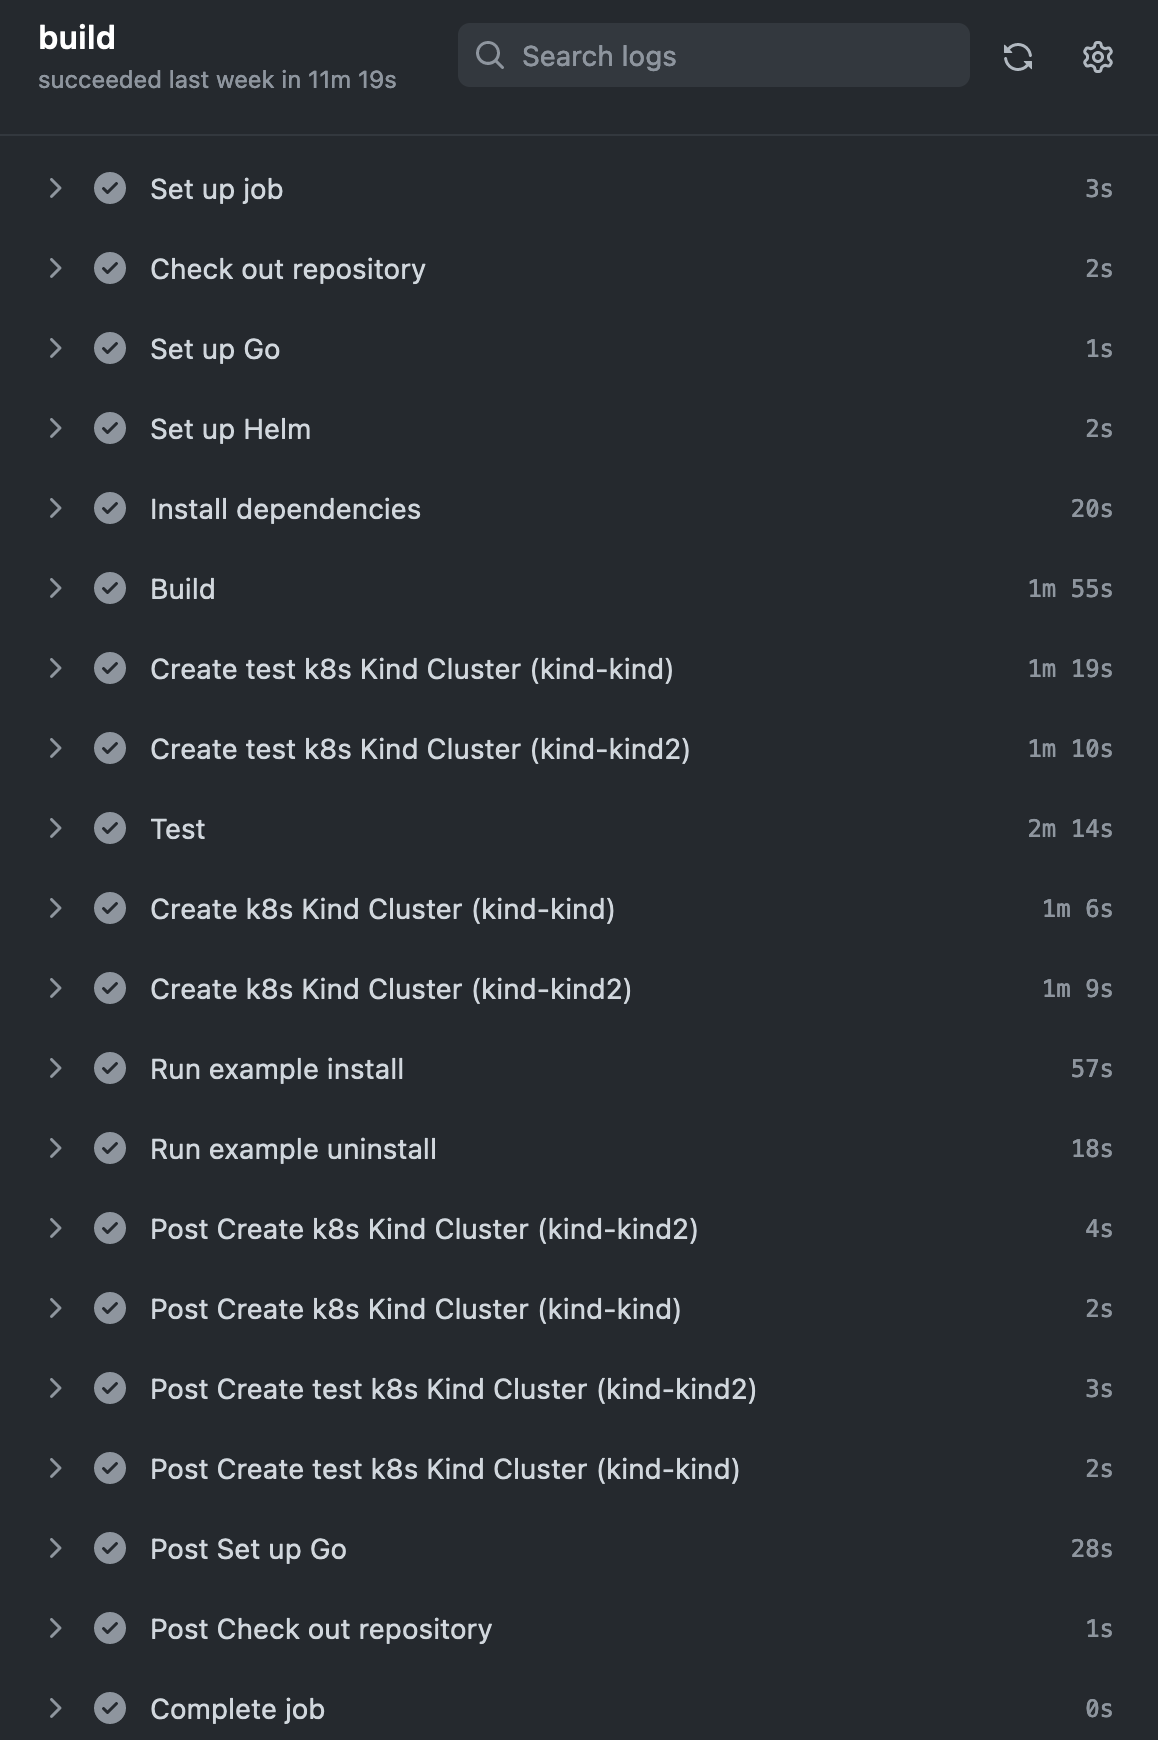
\includegraphics[width=0.65\textwidth]{figures/kli/actions-run-log.png}
        \caption{Sikeres GitHub Actions teszt kimenete.}
         \label{github-actions-run-log}
\end{figure}

\begin{figure}
  \centering
  \begin{minipage}{\linewidth}
      \begin{lstlisting}[language=go]
        func TestGetDeploymentName(t *testing.T) {
          createTestClient()
          resetCluster()
          setupCluster()
        
          _ = Apply(&testDeployment)
          WaitForReadyDeployment(testDeployment)
        
          deploymentName, err := GetDeploymentName(testDeploymentReleaseName, testNamespaceName)
          if err != nil {
            t.Error(err.Error())
          }
        
          if testDeploymentName != deploymentName {
            t.Error("Deployment name is wrong!")
          }
        }
      \end{lstlisting}
  \end{minipage}
  \caption{Kódrészlet az egyik teszt függvényről.}
    \label{test-code-snippet}
\end{figure}

\section{Kritikai elemzése}
A program kritikus szemmel nézve kifogásolható több ponton is.
Ez betudható a tervezésem pontatlanságának és a kivitelezési megoldásomban.
Ezekre a pontatlanságokra fogok rávilágítani a következő pár szekcióban.

\subsection*{Felhasználói felület}
A felhasználói felületen megjelenő üzenetek sok helyet igényelnek és lehetnének informatívabbak az aktuális folyamat állapotáról.
Jelenleg minden üzenetet új sorban ír ki a konzolos applikáció, mely hamar betelíti a konzolos ablakot és nehezen visszakereshetővé teszi az üzeneteket.
Ezt a problémát lehet orvosolni, ha csoportosítom logikailag a folyamatok lépéseit és az egy csoportba tartozó lépéseket egy sorba írom ki, felülírva mindig az előző üzenetet. Ezzel sokkal kevesebb kiírás fog megtörténni és a folyamat végeredménye könnyen követhető lesz.

Ezáltal, hogy kevesebb kiírás fog megmaradni a képernyőn megnyílik a lehetőség több információ megjelenítésére.
Ezek az információk segítenének a felhasználónak a hibák felderítésében és a folyamat várható befejezési idejének meghatározásában.

A flag-ek kiosztása nem eléggé intuitív és konzisztens. Kevés betű van használatban, így könnyen keverhetőek egymással a flag-ek.
Több funkció esetében még nagyon problémává növi ki magát.

\subsection*{Megvalósítás}
A kód minőségén lehetne javítani többféle képpen is, ezzel segítve a későbbi módosítások elvégzését.
A függvények és változók elnevezése nem mindig teljesen reprezentatív, a kódolási stílus változó.
Bár ezek többsége ízlés kérdése is, érdemes használnom a későbbiekben go linter-eket, melyek segítenek elemezni a kódot és akár javítási javaslatot is tesznek. Ezzel könnyedén elérhetővé válik az egységes kód, mely akkor is az marad, mikor több ember dolgozik rajta. 

Helm konfig fájl beolvasásáért felelős kódrészlet nem az io csomagban található annak ellenére, hogy semmi függősége nincs a helm-hez.
Ez a kódrészlet a program kezdeti fázisában lett megírva és nem lett átmozgatva az io csomagba.

\section{Továbbfejlesztési lehetőségek}
Ennek a CLI programnak a továbbfejlesztését úgy képzelem el, hogy olyan funkciók kerülnek implementálásra, melyek segítenek a felhasználónak az Istio operátor telepítésében.

\subsection{Operátor frissítése}
Az Istio operátor telepítése után nincs mód annak frissítésére a programom keresztül.
Ehhez segítségül kell hívni a helm parancsot, melyet a felhasználó lehet, hogy nem ismer.
Mivel a programom felhasználóbarát megoldásokat kínál, így magától adódik ennek a funckiónak az automatizálása.
Meglévő klaszter telepítésnél lehetőség adódna frissíteni a komponenseket egy adott verziószámra.
Ez a verziószám lehetne a legfrissebb kiadás, de régebbi verziók is rendelkezésre állnának.

A megvalósítása ennek egyszerű feladat, ugyanis már implementálva van egy helm kliens mely feltelepíti az istio operátort.
Ennek a kliensnek van chart frissítési funkciója is, így csak azt kell meghívni a kódomban.
Ehhez a funkcióhoz be kell vezetnem egy új parancsot (nevezzük upgrade-nek).
Az upgrade parancsnak flag-eken keresztül meg kellene adni, hogy melyik resource-t szeretnénk frissíteni.
Ezután egy listából kiválaszthatjuk a telepíteni kívánt verziót. Ezeket a verziószámokat egy webes kérés segítségével lekérdezhető az internetről.

\subsection{Log rendszer}
Az automatizálás részeként kiegészíteném egy log rendszerrel a programomat, így felügyelet nélkül lehet hagyni a programot futtatás közben.
Ehhez létrehoznék egy \texttt{-{}-}log (vagy röviden -l) flag-ek, melynek egy elérési útvonalat lehetne átadni, ahol létrehozna egy szöveges fájlt és beleírná a telepítési eseményeket. Előre meg lehetne határozni több szintű log-olási részletességet és lehetőség adódna a standard output-ra való kiírás minimalizálására is.
A log fájl jól struktúrált lenne, ami segítené automatizálhatóan feldolgozni és visszanézhetővé tenni a telepítési folyamat sikerességét.
Előnye fájlba log-olásnak, hogy sokkal több részletet lehetne leírni az adott folyamatról vagy annak hibájáról, míg ez a részletesség a standard output-on zavaró lehet.

Implementálását úgy oldanám meg, hogy létrehoznék egy saját kiíró függvényt (nevezzük printer-nek) az io csomagban.
Ebben printer függvényben lenne egy ellenőrző logika, hogy az adott \texttt{-{}-}log (vagy röviden -l) flag használatban van-e és ennek megfelelően írja ki az eseményeket. Minden kiírásért felelő függvényemet lecserélném a printer függvényre és készen is van a funkció. 

\subsection{Virtuálisgép integráció megvalósítása}
Vannak olyan workload-ok, melyek jobban teljesítenek monolitikus applikációként és negatív hatással lenne rá a mikroszolgáltatási struktúra.
Erre kínálnék megoldást a virtuális gép integrációval.
Ehhez szükség lenne hozzáadni kettő új parancsot a cobra cli alkalmazásomhoz:
\begin{itemize}
  \item Az egyik parancs (nevezzük serve-nek) felelne a virtuális gép beállításáért, hogy tudjon kommunikálni majd a cluster-el.
  \item A másik parancs (nevezzük connect-nek) felelne a virtuális gép hozzáadásáért a meglévő cluster-hez.
\end{itemize}

A serve parancs egy szolgáltatásként futna a virtuális gépen, melyet REST API hívások segítségével lehetne elérni.
Ezekkel a hívásokkal adatokat és parancsokat lehetne küldeni a virtuális gépnek, amik feldolgozásra kerülnének.

A connect parancs létrehozna egy deployment típusú erőforrást a cluster-en, melyben konfigurálva lenne egy kliens a REST API kommunikációhoz.
Ezt a klienst egy webszerveren keresztül elérhetővé tenném hasonlóan egy dashboard-hoz, ahol látható lenne statisztika a virtuális gépről és parancsokat lehetne küldeni.

\subsection{Klaszterek létrehozása telepítés előtt}
Mivel minden népszerű felhőszolgáltató kínál lehetőséget API-on keresztül létrehozni cluster-eket, így egyszerű lenne ennek a funkciónak az implementálása.
A felhasználónak lehetősége lenne létrehozni előre definiált cluster-eket egy konfigurációs fájl segítségével.
Ez a konfigurációs fájl leírná a cluster szolgáltatóját, az azonosításhoz szükséges adatokat, a cluster méretét és fajtáját.
Egy \texttt{-{}-}setup (vagy röviden -s) flag bevezetését követően át lehet adni a programnak az elérési útvonalát a konfigurációs fájlnak.
Ebből az adatokat kiolvasva létre lehet hozni egy klienst, mely az API kéréseket fogja létrehozni.

\newpage

\subsection{Automatizált post-install}
Miután megtörtént a telepítés és attach, lehetőség lenne kiválasztani a menüből előre összeállított vagy egyedileg definiált deploymenteket és helm chart-ok telepítésére.
A post-install konfigurációs leíró fájlt meg lehetne adni egy flag-el, így teljesen automatikusan futna le a teljes folyamat.
A felkínált post-install lista olyan elemeket tartalmazna, melyek nagy segítséget nyújthatnak a klaszter további üzemeltetésében.
Előre összeállított deploymentekre példák:
\begin{itemize}
    \item Kubernetes dashboard telepítése.
    \item Prometheus monitorozó rendszer beállítása.
    \item Grafana dashboard telepítése.
    \item cert-manager TLS cert manager konfigurálása.
\end{itemize}
